\chapter{RSS Indoor localization}\label{sec:RSSIndoorLocalization}
This chapter describes most common techniques and methods for indoor localization using radio signal strength (RSS).

\section{Triangulation}\label{sec:Triangulation}
Methods based on Triangulation use geometric properties of triangles to determine target position. This can further be divided into lateration and angulation. \cite{RAinWILTaS} There are multiple sources of data these methods can use like distance estimation between device and specific transmitters, measurements of the signal propagation-time (TOA: Time Of Arrival and TDOA: Time Difference of Arrival\cite{LTinWSN}) and the direction of received
signal (AOA: Angle of Arrival\cite{AoALforWSN}).

\subsection{Lateration}\label{sec:Lateration}
Lateration refers to the technique of determining position based on distance measurement. There are two main types of lateration and those are Trilateration and Multilateration. 

\subparagraph{Trilateration} uses distance data from multiple reference points, at least 3 in particular as "tri" in the name suggests.\cite{RAinWILTaS} This technique can be used in 2D and 3D plane. 

\begin{figure}[h!]
	\begin{centering}
		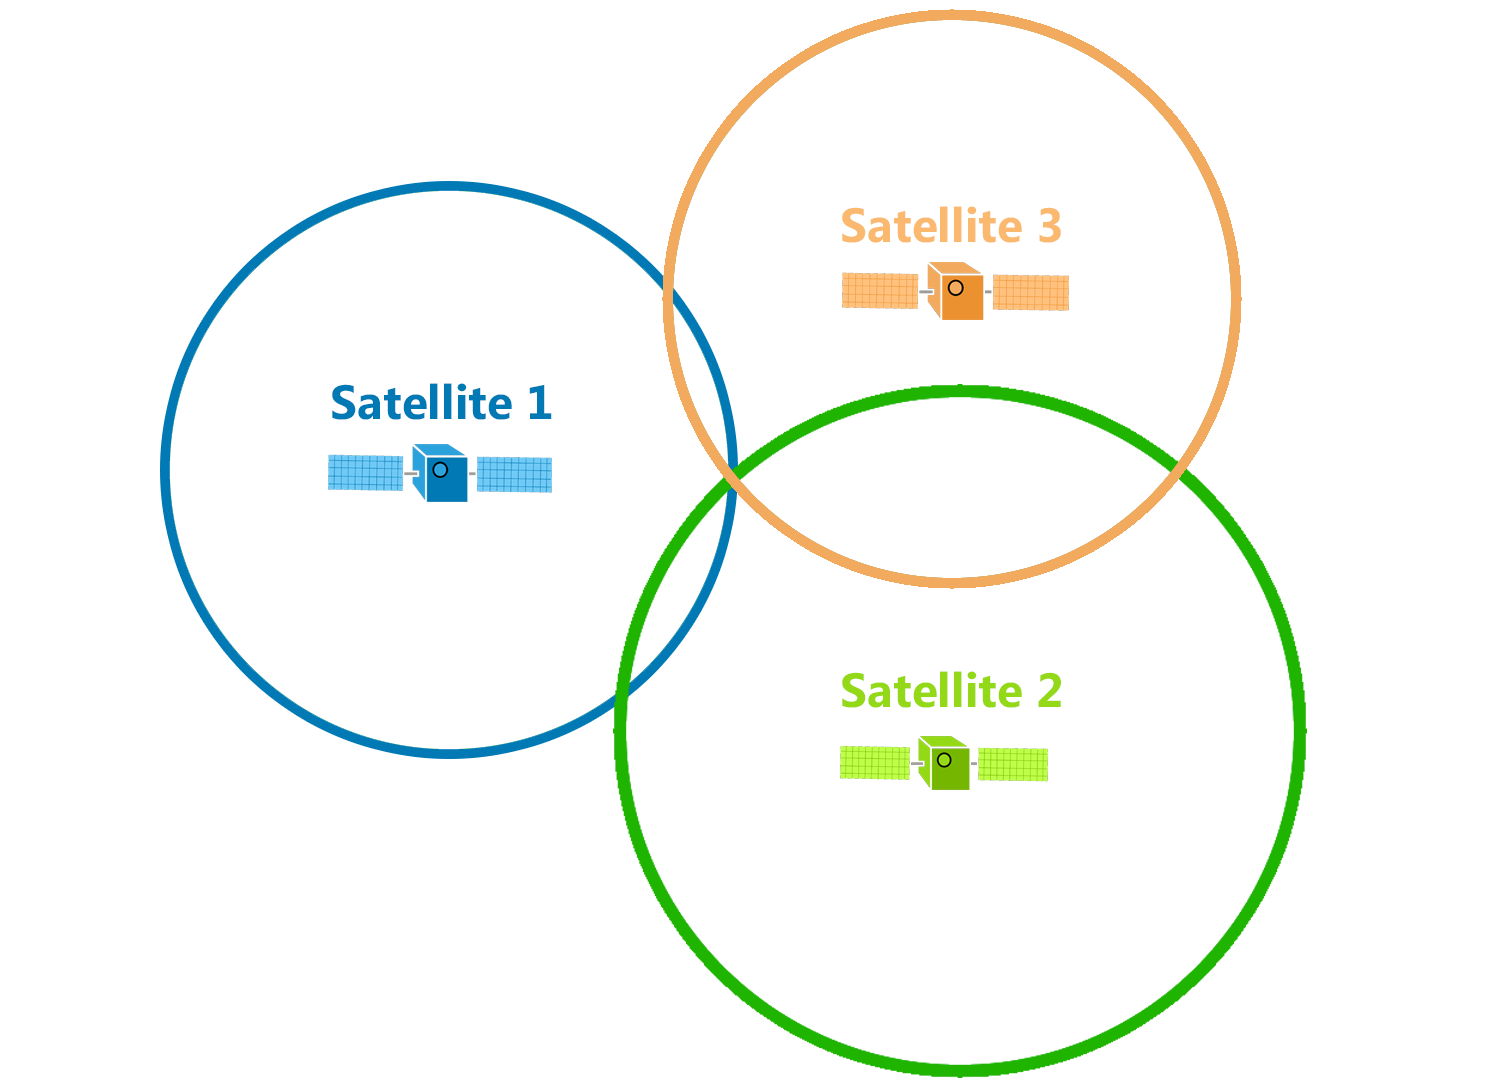
\includegraphics[width=0.48\textwidth]{img/trilateration_2d}
		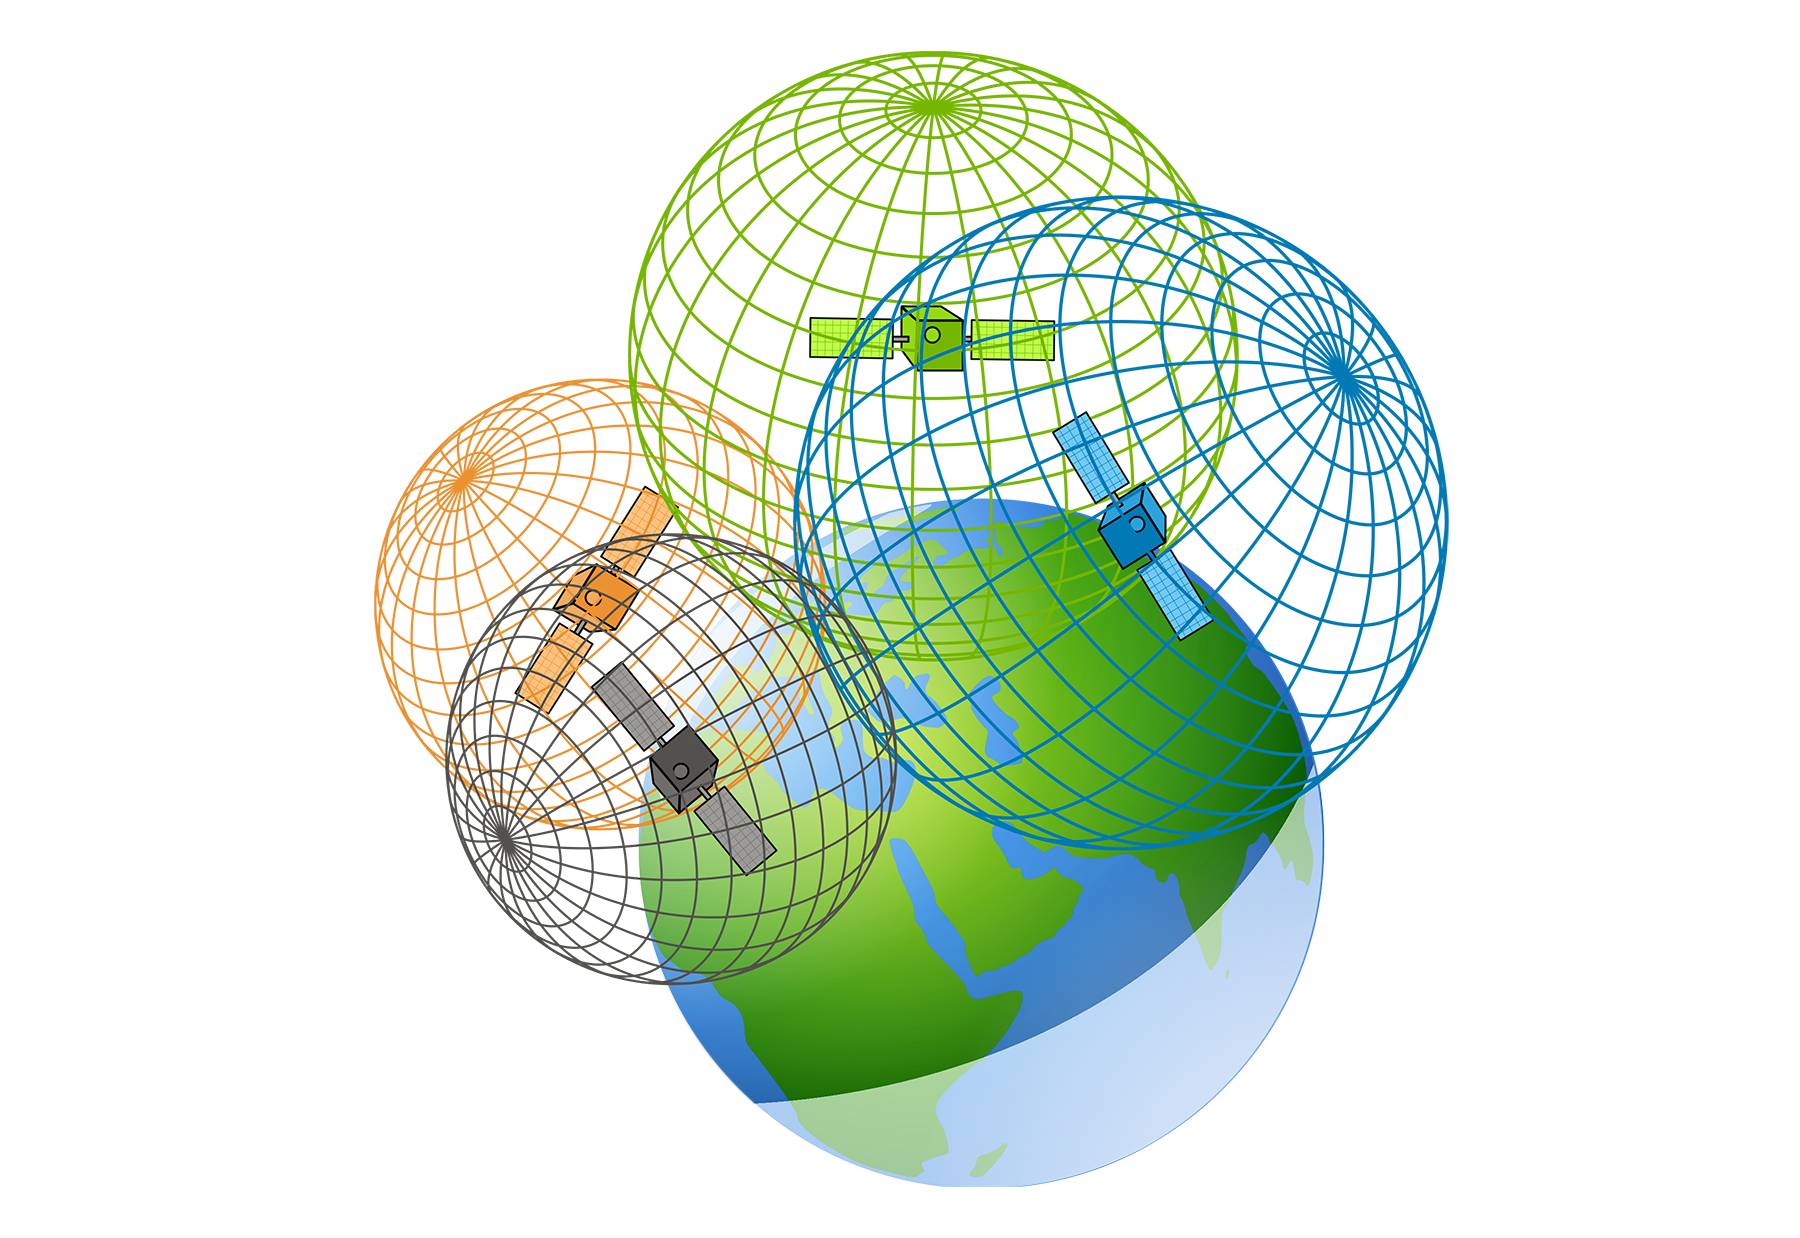
\includegraphics[width=0.48\textwidth]{img/trilateration_3d}
		\par\end{centering}
	\caption{2D and 3D Trilateration (source: \cite{TvTHGPSRW})\label{fig:2d_and_3d_trilateration}}
	\label{fig2}
\end{figure}

\fref{fig2} illustrates usage of Trilateration in 2D and 3D environment. While working in 2D plane will result with only one specific location point. Moving to the 3D plane creates a problem because signal is send in a sphere which will result in two positions instead of one. That is the reason why there is the need to add fourth data source for single position calculation.

Multilateration


\subsection{Angulation}\label{sec:Angulation}

\section{Fingerprinting}\label{sec:Fingerprinting}
This method is a part of already mentioned Signal Strength Fingerprint Maps (SSFM) type. Main point of this method is using previously recorded data to figure out location inside the building. Hence fingerprint term in the name. There is multiple kinds of data that can be recorded like magnetic field strength or light signals but as it was already mentioned this topic is focused RSS. There are also multiple sources of radio signals like bluetooth, wireless or cellular devices and networks.

This method has two main stages where the first one is fingerprint maps construction also called offline stage. They are created using collecting Received Signal Strength (RSS) at different positions with specific coordinates of this place. All fingerprints are saved in the database and this is called fingerprint map. The other part is localization stage also known as online stage where client device measures data and compares them with fingerprint maps to approximate position. \cite{LocalizationApproaches}\cite{IndoorLocalizationWithoutThePain}

\section{Proximity}\label{sec:Proximity}
Proximity detection also knows as connectivity based positioning is one of the simplest method to implement.

\section{Other techniques}
%\section{Dead Reckoning}\label{sec:DeadReckoning}

%\section{K neighbors}\label{sec:KNeighbors}

%\section{Compressive sensing}\label{sec:CompressiveSensing}